\documentclass[conference]{IEEEtran}
\IEEEoverridecommandlockouts
% The preceding line is only needed to identify funding in the first footnote. If that is unneeded, please comment it out.
\usepackage{cite}
\usepackage{amsmath,amssymb,amsfonts}
\usepackage{algorithmic}
\usepackage{algorithm}
\usepackage{graphicx}
\usepackage{textcomp}
\usepackage{xcolor}
\usepackage{booktabs}
\usepackage{tikz}
\usetikzlibrary{positioning,arrows.meta,trees,shapes.geometric,calc}
\usepackage[hidelinks]{hyperref}
\newcommand{\rvr}{\textsuperscript{$\dagger$}}
\def\BibTeX{{\rm B\kern-.05em{\sc i\kern-.025em b}\kern-.08em
    T\kern-.1667em\lower.7ex\hbox{E}\kern-.125emX}}
\begin{document}

\title{Business Analytics for Audit and Fraud Detection: An Integrative Review of Digital Tools, a Red-Flag Taxonomy and a Conceptual AI-Assisted Prioritisation Framework\\


}

\author{
    \IEEEauthorblockN{
        Author Name\textsuperscript{1}
    }
    \IEEEauthorblockA{
        \textsuperscript{1}Department, Institution, City, Country\\
        Email: author@example.com
    }
}

\maketitle

\begin{abstract}
Business analytics (BA) and AI are increasingly proposed to strengthen audit and fraud detection, yet evidence on digital audit tools, red-flag indicators and the organisational conditions under which analytics delivers value remains fragmented across technical, accounting and practitioner literatures. This paper reports an integrative review that synthesises this fragmented evidence and develops a coherent conceptual framework linking audit-analytics capabilities, a red-flag indicator taxonomy and an AI-assisted prioritisation procedure. Using an integrative-review design with a PRISMA-informed screening protocol, 84 sources---peer-reviewed articles, industry reports and professional publications published between 2015 and 2025---were coded against five audit-model dimensions and synthesised thematically. The synthesis indicates that analytics can extend audit coverage from sampling to population-level testing and can support continuous and predictive assurance, while reported benefits depend strongly on data quality, analytical skills and governance, which the reviewed literature identifies as recurring obstacles. The review offers three synthesised contributions: (i) ~a five-cluster red-flag taxonomy aligned with corresponding analytical techniques; (ii) ~a comparative synthesis of five audit-analytics platforms and an analytics-maturity model; and (iii) ~a model-agnostic, conceptual AI-assisted red-flag prioritisation framework expressed as a weighted risk score and a reviewable prioritisation procedure. The prioritisation framework is conceptual: it is a synthesis-driven proposal and is not empirically validated in this study, and no accuracy, precision or recall figures are claimed for it. For practitioners, the synthesis provides a structured basis for tool selection, for sequencing analytics maturity and for governing algorithmic outputs; for researchers, it identifies empirical validation of such frameworks as an open priority.
\end{abstract}

\begin{IEEEkeywords}
Business Analytics, Audit Automation, Fraud Detection, Red-Flag Indicators, Integrative Review, AI-Assisted Prioritisation, Analytics Maturity
\end{IEEEkeywords}

\section{Introduction}

The rapid digitalisation of financial systems has reshaped auditing by generating volumes of accounting data that traditional audit methods cannot readily process \cite{b1}. Conventional auditing, based on periodic review cycles, human judgment and selective sampling, was designed for a less complex era in which financial records were fewer, more stable and less prone to manipulation \cite{b2}. In modern organisations, manual audit methods typically scrutinise only a limited subset of transactions, which allows misstatement in large transaction populations to remain undetected for prolonged periods and, in some cases, to be discovered only after significant loss \cite{b3}. These methods also struggle to detect subtle, deliberately concealed alterations in financial records and therefore may not provide the timely assurance that contemporary business cycles require. As financial crime becomes harder to identify because of digital payment systems, complex vendor networks and dispersed data, conventional audit methods may become a governance risk in themselves \cite{b4,b5}.

Business analytics (BA) has been proposed as a response to these structural constraints, shifting assurance from reactive and periodic testing towards proactive, continuous and data-driven practice \cite{b6,b7}. By enabling examination of complete transaction populations rather than samples, BA allows auditors to surface anomalies, behavioural irregularities and structural inconsistencies at scale. Machine learning, predictive risk models, network analysis and natural language processing have been reported to extend auditors' detection capabilities to indicators such as irregular journal entries, atypical vendor relationships and after-hours access, which may precede or accompany fraudulent activity \cite{b8,b9,b10}. The reviewed literature reports that organisations adopting analytics-driven auditing tend to observe improved detection outcomes relative to conventional techniques, alongside reductions in false positives attributable to machine-learning-based anomaly detection \cite{b11,b4}; the magnitude of these gains varies considerably with data quality and deployment context.

Despite this promise, existing research on BA in auditing remains fragmented in several respects. There is limited comparative evidence on the relative effectiveness of different analytical methods---for example supervised versus unsupervised learning---across audit contexts and fraud types. Guidance on practical implementation is sparse, particularly regarding change management, workflow integration and the hybrid competencies that combine accounting expertise with data-science skills. Moreover, much of the literature adopts narrow perspectives, examining a specific technology, a single industry case or a technical performance metric in isolation from the organisational and ethical challenges of implementation \cite{b12}. As a result, practitioners face uncertainty about tool selection, integration into existing audit processes, algorithmic bias and transparency, and the consequences of analytics for audit quality and professional scepticism. A synthesis that connects these strands is therefore needed.

These gaps carry implications for several stakeholder groups, which motivates this review. The absence of established implementation standards leads to inconsistent adoption and can undermine confidence in algorithmic outputs, while the lack of uniform standards for algorithmic auditing poses regulatory challenges as analytics spreads across global assurance practice. The gap between current curricula and the hybrid skills auditors require affects graduates' readiness for data-driven practice \cite{b13}. As expectations and oversight increase, analytical capability becomes important for maintaining the relevance and value of audit operations \cite{b14}. Finally, the scarcity of a connected conceptual framework means that empirical studies in this area proceed without a common structure, limiting comparability.

Against this background, this review addresses four research questions:
\begin{itemize}
    \item \textbf{RQ1:} Which analytical methods and digital tools does the reviewed literature apply to audit and fraud detection, and with what reported capabilities and limitations?
    \item \textbf{RQ2:} How can red-flag indicators be classified into a coherent taxonomy that links each class to appropriate analytical techniques?
    \item \textbf{RQ3:} How do analytical maturity, tool choice, sector and organisational readiness condition the realisation of analytics benefits in audit?
    \item \textbf{RQ4:} What conceptual framework can integrate a red-flag taxonomy, analytics capabilities and AI-assisted prioritisation into the audit workflow, and what remains to be empirically validated?
\end{itemize}

To address these questions, the study undertakes a qualitative integrative review of 84 sources drawn from peer-reviewed articles, industry reports and professional publications published between 2015 and 2025. The synthesis suggests that although analytics offers demonstrable advantages in coverage and timeliness, its effective application is constrained by data-quality deficiencies repeatedly identified as the primary obstacle \cite{b15}, skill gaps within audit teams \cite{b16} and ethical concerns surrounding AI-generated insight and imbalance \cite{b17}. Adoption differs across sectors: regulated financial institutions are among the most advanced adopters, driven largely by regulatory pressure, whereas small and medium-sized enterprises lag because of resource and capacity constraints \cite{b18,b19}. Network analysis is reported to strengthen forensic investigation \cite{b20}, and regulators increasingly use analytics for systemic risk monitoring and compliance trend analysis \cite{b21}.

The review makes the following contributions:
\begin{itemize}
    \item \textbf{C1 (methodological):} a documented, PRISMA-informed integrative-review protocol (search, screening, coding and triangulation) that makes the synthesis and its limitations auditable, with points requiring author confirmation explicitly flagged.
    \item \textbf{C2 (conceptual):} a five-cluster red-flag taxonomy in which each class is defined and linked to the analytical techniques that are reported to detect it, distinguishing categories conceptually so that they do not substantially overlap.
    \item \textbf{C3 (comparative):} a synthesis of five audit-analytics platforms across shared dimensions together with an analytics-maturity model that connects descriptive-to-prescriptive capability with data, technology, workforce, governance and explainability conditions.
    \item \textbf{C4 (framework):} a model-agnostic, conceptual AI-assisted red-flag prioritisation framework, expressed as a weighted risk score and a reviewable procedure, positioned explicitly as a proposal for future empirical testing rather than a validated model.
\end{itemize}

The remainder of the paper is organised as follows. Section~\ref{sec:method} describes the review methodology. Section~\ref{sec:results} synthesises the findings and discusses their implications. Section~\ref{sec:conclusion} presents conclusions, policy implications and limitations, and identifies priorities for future research.

\section{Methodology}
\label{sec:method}

This section describes the review protocol. It first sets out the theoretical lenses adopted, then the review design, search and screening strategy, coding and synthesis procedure, and finally the analytical frameworks used to organise the synthesis (an audit-model comparison, a tool categorisation, a red-flag taxonomy and a conceptual prioritisation framework).

\subsection{Theoretical Foundations}

Three established theoretical lenses guide the synthesis. First, the Fraud Triangle explains fraud as the convergence of pressure (incentive), opportunity and rationalisation \cite{b66}. Audit analytics bears primarily on the opportunity element, by continuously exposing control weaknesses and anomalous transactions, and secondarily on pressure, by supplying early-warning signals; the taxonomy in Section~\ref{sec:taxonomy} is organised around observable indicators of these elements. Second, the Technology--Organization--Environment (TOE) framework is used to explain uneven adoption, distinguishing technological readiness, organisational capability (skills, governance, change management) and environmental factors such as regulation and competitive pressure \cite{b67}. Third, an analytics-maturity perspective, spanning descriptive, diagnostic, predictive and prescriptive capability, provides a developmental scale against which reported detection capability is assessed in Section~\ref{sec:maturity}. Together these lenses connect the reviewed tools and red-flag indicators to established explanations of fraudulent behaviour and of organisational technology adoption. They are used to structure interpretation; they are not tested empirically here.

\subsection{Review Design and Analytical Strategy}

The review follows an integrative design rather than a systematic review, because the aim is to synthesise heterogeneous evidence---empirical studies, conceptual frameworks, industry reports and practitioner guidance---into a coherent account, emphasising interpretation over statistical pooling. Integrative reviews are appropriate where the literature is methodologically diverse and where the objective is conceptual synthesis rather than effect estimation. The design is qualitative and interpretive: audit tools and red-flag indicators are treated as acquiring meaning and effectiveness through their position within particular institutional, technological and cultural configurations, rather than as context-free instruments. This interpretive stance is adopted deliberately and is reflected in the limitations in Section~\ref{sec:limitations}.

\subsection{Search Strategy and Source Selection}

A multi-stage retrieval strategy was used to assemble academic and professional literature on audit analytics and fraud detection. Thematic accuracy was pursued through purposive sampling with iterative refinement of search terms. Keyword groups spanned audit automation, fraud analytics, continuous auditing, anomaly detection in finance and digital auditing frameworks, together with related terms.

Sources were retrieved from five databases: Scopus (n = 64), Web of Science (n = 41), IEEE Xplore (n = 36), SSRN (n = 58) and Google Scholar (n = 73), a combined total of 272 records for the period 2015--2025. In addition, 25 industry reports and white papers issued by ISACA and the Big Four accounting firms were included to complement academic evidence with practitioner perspectives. Records were screened in two stages: title and abstract review, followed by full-text review. The arithmetic of the selection process is summarised in Table~\ref{tab:protocol} and is internally consistent (272 academic + 25 professional = 297 retrieved; 25 duplicates removed = 272; 118 excluded at title/abstract = 154; 70 excluded at full text = 84 included).

Inclusion required that a source (i) address digital auditing, audit analytics or fraud analytics; (ii) display sufficient methodological or procedural transparency to permit appraisal; and (iii) offer practical relevance to organisational or audit decision-making. Sources were excluded if they were editorial or non-substantive, lacked clarity in execution, or addressed non-financial topics. To avoid presenting academic and professional evidence as equivalent, sources were tagged by type at the coding stage so that claims resting on grey literature could be distinguished from those supported by peer-reviewed research.

% [AUTHOR INPUT REQUIRED: insert the exact database search strings and the date of the final search here. Kept out of the compiled text so the PDF reads cleanly; tracked in revision_report.md.]
% [AUTHOR INPUT REQUIRED: state whether title/abstract and full-text screening were performed by one reviewer or independently by multiple reviewers, and inter-rater agreement if applicable.]
% [AUTHOR INPUT REQUIRED: state the screening/reference-management software used (e.g., Covidence, Rayyan, Zotero) and the final split of the 84 included sources into peer-reviewed articles vs industry/professional reports.]

\begin{table}[!t]
\caption{Review Protocol and Source Selection}
\label{tab:protocol}
\centering
\footnotesize
\begin{tabular}{p{0.40\columnwidth} p{0.15\columnwidth} p{0.28\columnwidth}}
\toprule
\textbf{Stage} & \textbf{Count} & \textbf{Note} \\
\midrule
Records retrieved (5 databases) & 272 & Scopus, Web of Science, IEEE Xplore, SSRN, Google Scholar \\
Additional professional sources & 25 & ISACA and Big Four reports \\
Total initially retrieved & 297 & \\
Duplicates removed & 25 & Overlap across databases \\
Records after de-duplication & 272 & Eligible for screening \\
Excluded at title/abstract & 118 & Out of scope or non-substantive \\
Excluded at full text & 70 & Editorial, low rigor, or off-topic \\
Included in synthesis & 84 & Tagged by source type \\
\bottomrule
\end{tabular}
\end{table}

\subsection{Coding, Synthesis and Validation Protocol}

Coding followed the three-stage thematic-synthesis approach of Thomas and Harden: line-by-line coding of each source to extract features, red-flag indicators, implementation challenges and value claims; consolidation of initial codes into descriptive themes; and development of analytical themes that connect these into an interpretive framework. Coding was iterative, and the codebook was reviewed and refined across analytical cycles to improve thematic consistency across document types. Further sources were added only until new themes ceased to emerge.

Findings were triangulated by contrasting academic evidence with the practices reported by the Big Four firms, by checking claimed tool functionality against publicly available documentation, and by relating red-flag typologies to case narratives in forensic accounting reports. Triangulation was used to strengthen interpretation; it does not convert the synthesis into an empirical validation.

% [AUTHOR INPUT REQUIRED: state the number of coders, whether coding was double-checked, and any measure of coding reliability. Tracked in revision_report.md.]

\subsection{Comparative Framework for Audit Models}

Audit models were compared along five dimensions: data coverage, audit timing, detection responsiveness, resource intensity and fraud traceability. These dimensions were derived from the reviewed literature and industry guidance and served as coding categories. Table~\ref{tab:framework} contrasts conventional and analytics-enabled auditing along these dimensions. Each included source was assessed for alignment with this framework, which provided a consistent basis for comparison and for identifying transition patterns from conventional to analytics-enabled practice.

\begin{table}[!t]
\caption{Comparative Framework: Conventional versus Analytics-Enabled Auditing}
\label{tab:framework}
\centering
\footnotesize
\begin{tabular}{p{0.18\columnwidth} p{0.33\columnwidth} p{0.33\columnwidth}}
\toprule
\textbf{Dimension} & \textbf{Conventional Auditing} & \textbf{Analytics-Enabled Auditing} \\
\midrule
Data coverage & Sample-based, with restricted visibility. & Population-level testing of complete datasets \cite{b22}. \\
Audit timing & Periodic, typically annual or quarterly. & Continuous or near-real-time procedures \cite{b23}. \\
Detection response & Post-event and reactive. & Real-time or predictive identification for pre-emptive action \cite{b24}. \\
Resource intensity & Labour-intensive and manual. & Automation can reduce manual effort \cite{b60}. \\
Fraud traceability & Limited, owing to fragmented records. & Improved, through auditable digital records \cite{b25}. \\
\bottomrule
\end{tabular}
\end{table}

\subsection{Tool Categorisation and Functional Analysis}

Five platforms frequently cited in academic and commercial sources were examined: ACL, IDEA, Power BI, Tableau, and open-source analytics (Python and R, treated together as one category because the reviewed sources discuss them jointly). Table~\ref{tab:tools} compares them across dimensions shared by the sources: primary audit application, data integration, visualisation, fraud/anomaly detection support, ease of adoption and principal limitation. The comparison is deliberately restricted to dimensions on which the reviewed sources report; no claims are made about capabilities outside this evidence base.

\begin{table*}[!t]
\caption{Comparative Analysis of Audit-Analytics Platforms (Open-Source = Python/R)}
\label{tab:tools}
\centering
\scriptsize
\setlength{\tabcolsep}{4pt}
\begin{tabular}{p{0.08\textwidth} p{0.15\textwidth} p{0.12\textwidth} p{0.10\textwidth} p{0.15\textwidth} p{0.11\textwidth} p{0.13\textwidth}}
\toprule
\textbf{Platform} & \textbf{Primary audit application} & \textbf{Data integration} & \textbf{Visualisation} & \textbf{Fraud / anomaly detection} & \textbf{Ease of adoption} & \textbf{Principal limitation} \\
\midrule
ACL & Structured audit tests and standardised reporting & Moderate, diverse datasets & Basic & Moderate, for irregularities & Easy for basic use & Limited advanced detection \cite{b26} \\
IDEA & File-consistency checks, fuzzy matching, regression-based anomaly identification & High, across formats & Adequate & Strong suitability for fraud identification & Moderate, training needed & Less flexible analytic workflows \cite{b27} \\
Power BI & Interactive financial dashboards and visual exploration & Robust, multi-source & High, interactive & Moderate; no native fraud models & Relatively easy & Limited inherent fraud detection \cite{b28} \\
Tableau & Visual analytics of financial data & Robust, seamless & Very high & Limited direct utility for fraud detection & Intuitive & Limited inherent fraud detection \cite{b29} \\
Python / R & Custom, reproducible analytics and modelling & Strong and scalable & Customisable & High, for complex analytics (reported) & Steep learning curve & Requires programming skill; no built-in audit interface \cite{b30} \\
\bottomrule
\end{tabular}
\end{table*}

The comparison suggests a trade-off between analytical power and accessibility: open-source platforms are reported as the most flexible for complex fraud analytics, whereas ACL, IDEA, Power BI and Tableau trade some analytical depth for usability, structured reporting or visual exploration. No single platform was reported as universally preferable; selection appears to depend on the audit objective, the team's competencies and the available data infrastructure \cite{b12}.

\subsection{Red-Flag Indicator Taxonomy}
\label{sec:taxonomy}

Red-flag indicators are observable signals that warrant audit attention. This review organises them into five clusters that are intended to be conceptually distinct: transaction irregularities, behavioural anomalies, structural anomalies, documentation discrepancies and relational fraud patterns. Unlike a simple list, each cluster is defined, illustrated, linked to the analytical techniques reported to detect it, and characterised by its limitations (Table~\ref{tab:taxonomy}). Figure~\ref{fig:taxonomy} presents the taxonomy conceptually. The clusters are not assumed to be exhaustive, and indicators may co-occur across clusters---an observation that motivates the combined prioritisation framework in Section~\ref{sec:framework}.

\begin{table*}[!t]
\caption{Five-Cluster Red-Flag Indicator Taxonomy}
\label{tab:taxonomy}
\centering
\scriptsize
\setlength{\tabcolsep}{4pt}
\begin{tabular}{p{0.12\textwidth} p{0.18\textwidth} p{0.15\textwidth} p{0.15\textwidth} p{0.15\textwidth} p{0.12\textwidth}}
\toprule
\textbf{Cluster} & \textbf{Definition (what it detects)} & \textbf{Representative indicators} & \textbf{Analytical techniques reported} & \textbf{Audit relevance} & \textbf{Limitations} \\
\midrule
Transaction irregularities & Deviations in timing, frequency, duplication or value of transactions & Duplicate payments; out-of-hours postings; unusual amounts & Rule-based tests; frequency and outlier detection; clustering & Detects possible control bypass in transaction processing & Prone to false positives; sensitive to threshold calibration \\
Behavioural anomalies & Deviations in user or entity behaviour relative to peers or history & Recurrent control violations; irregular access; resistance to oversight & Behavioural analytics; peer-group comparison; sequence mining & Early indication of insider or override risk & Requires reliable access-log data; privacy considerations \\
Structural anomalies & Inconsistencies in ledgers, reconciliations or reporting structures & Unbalanced accounts; incongruous reconciliations; unit inconsistencies & Statistical reconciliation; graph analysis of accounts & Signals weak control design and governance gaps & Requires integrated, well-modelled data \\
Documentation discrepancies & Manipulated, duplicated or unauthorised documents & Forged or duplicated invoices; unauthorised edits; altered dates & Duplicate and near-duplicate detection; OCR with NLP; metadata analysis & Addresses invoice authorisation and documentary integrity & Sensitive to data quality; can be concealed adversarially \\
Relational fraud patterns & Coordinated or collusive relationships among entities & Bid-rigging; related-party networks; circular payments & Graph/network analytics; community detection; link analysis & Surfaces schemes that evade rule-based tests & Data-intensive; interpretability and false-link risks \\
\bottomrule
\end{tabular}
\end{table*}

\begin{figure}[!t]
\centering
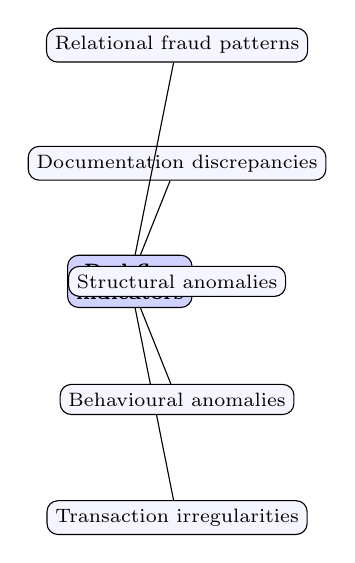
\begin{tikzpicture}[
  font=\scriptsize,
  grow=right,
  level distance=6mm,
  every node/.style={draw, rounded corners, align=left, inner sep=3pt, fill=blue!4},
  core/.style={fill=blue!18, font=\scriptsize\bfseries, align=center},
  edge from parent/.style={draw}]
\node[core] {Red-flag\\indicators}
  child { node {Transaction irregularities} }
  child { node {Behavioural anomalies} }
  child { node {Structural anomalies} }
  child { node {Documentation discrepancies} }
  child { node {Relational fraud patterns} };
\end{tikzpicture}
\caption{Five-cluster red-flag indicator taxonomy (conceptual synthesis; clusters are non-exhaustive and may co-occur).}
\label{fig:taxonomy}
\end{figure}

\subsection{Analytics-Driven Audit Workflow}
\label{sec:workflow}

The reviewed sources converge on a five-stage analytics workflow for audit: data collection, data preparation, exploratory modelling, risk scoring and red-flag issuance \cite{b58}. Figure~\ref{fig:workflow} presents this workflow conceptually. Data collection draws structured and unstructured financial data from enterprise resource planning systems, spreadsheets, transaction logs and internal communications. Data preparation---cleansing, de-duplication, transformation and normalisation---ensures that datasets are consistently formatted for analysis; the reviewed sources describe this stage as the most resource-intensive of the workflow. Exploratory modelling applies clustering, trend detection and outlier identification to surface latent relationships and irregularities \cite{b59}. Risk scoring assigns weighted values to the frequency and severity of anomalies to rank investigative tasks, and red-flag issuance produces alerts and visual summaries for auditor dashboards. The workflow is iterative rather than linear: insights from red-flag outputs feed back to refine data features and model parameters, and governance mechanisms align analytical activity with organisation-wide risk protocols.
% [NEEDS EVIDENCE: the source manuscript stated that data preparation consumes ~50% of effort; no cited source supports this figure, so it was removed. Reinstate only with a citation.]

\begin{figure*}[!t]
\centering
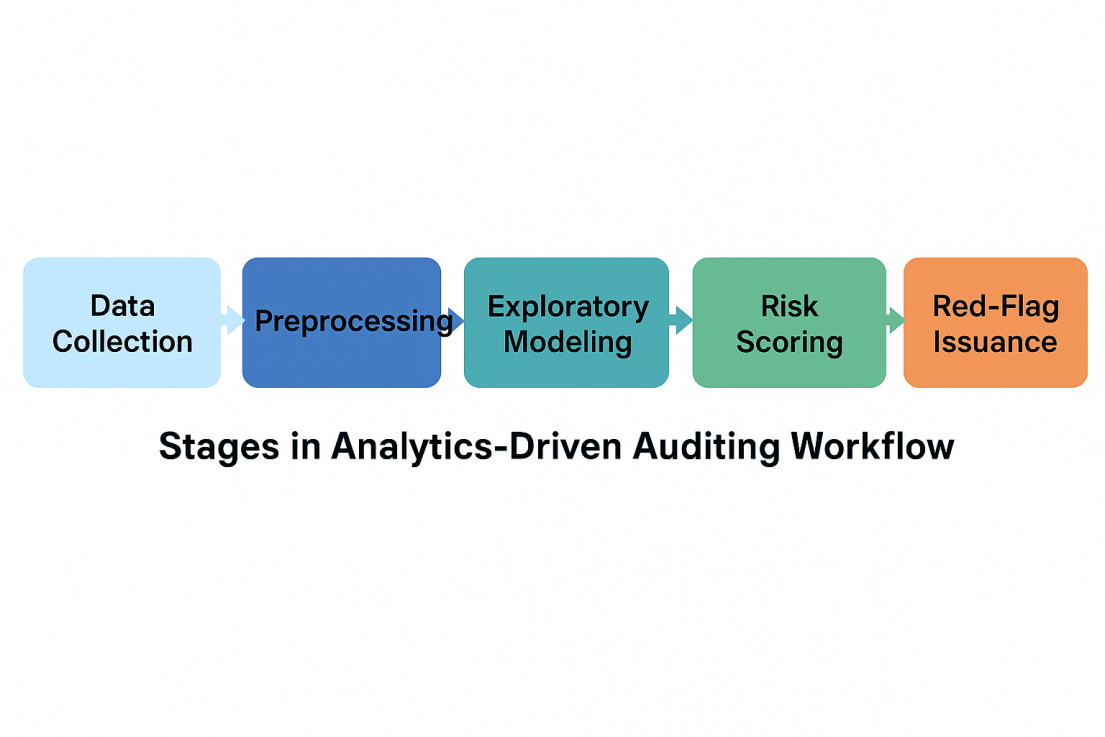
\includegraphics[width=0.8\textwidth]{figs/workflow.png}
\caption{Analytics-driven audit and fraud-detection workflow (five conceptual stages; described by the reviewed sources as the most resource-intensive phase, data preparation precedes modelling, scoring and red-flag issuance).}
\label{fig:workflow}
\end{figure*}

\subsection{AI-Assisted Red-Flag Prioritisation Framework}
\label{sec:framework}

Building on the workflow model and the taxonomy, this review consolidates the reported techniques into a conceptual, model-agnostic prioritisation framework. The purpose is to give a single interpretable score to each transaction or journal entry so that finite audit resources can be directed towards the most consequential cases. Let $x_r$ denote the feature vector of record $r$ (temporal, monetary, categorical and textual attributes). Four terms are combined, each normalised to $[0,1]$:
\begin{itemize}
    \item $a(x_r)$: an unsupervised anomaly score (for example from an isolation forest, an autoencoder or a clustering-distance measure);
    \item $b(x_r)$: a behavioural-deviation score relative to a peer group or the entity's own history;
    \item $c(x_r)\in\{0,1\}$: a binary indicator that record $r$ violates a defined control rule;
    \item $f(x_r)$: a normalised frequency/severity term capturing how often and how materially such an event occurs.
\end{itemize}

The composite risk score is
\begin{equation}
s(r)=w_1 a(x_r)+w_2 b(x_r)+w_3 c(x_r)+w_4 f(x_r),
\label{eq:risk}
\end{equation}
where the weights satisfy $w_i \ge 0$ and $\sum_{i=1}^{4} w_i = 1$. Because all terms are normalised to $[0,1]$ and the weights sum to one, $s(r)\in[0,1]$, which admits a single interpretable threshold $\tau$. Records with $s(r) > \tau$ are escalated for investigation, while records below $\tau$ enter routine monitoring; in practice $\tau$ should be calibrated against the auditor's relative tolerance for false positives and false negatives rather than fixed a priori. The weights encode the auditor's emphasis and risk appetite and, like $\tau$, require calibration on representative data. Algorithm~\ref{alg:redflag} summarises the procedure, which operationalises the anomaly-detection, risk-scoring and red-flag-issuance stages of the workflow. Figure~\ref{fig:prio} presents the framework conceptually.

\begin{algorithm}[!t]
\caption{AI-Assisted Red-Flag Prioritisation (Conceptual)}
\label{alg:redflag}
\begin{algorithmic}
\REQUIRE transaction data $D$, control rules $C$, weights $w$, threshold $\tau$
\ENSURE ranked red-flag list $L$
\STATE preprocess $D$ and engineer features (temporal, monetary, categorical, textual)
\FOR{each record $r \in D$}
    \STATE compute anomaly score $a(x_r)$ and behavioural score $b(x_r)$
    \STATE set $c(x_r)$ from control-rule engine $C$
    \STATE compute composite score $s(r)$ via Eq.~\eqref{eq:risk}
\ENDFOR
\STATE rank $D$ by $s(r)$ in descending order
\FOR{each record $r$ with $s(r) > \tau$}
    \STATE assign red-flag cluster from the taxonomy (Table~\ref{tab:taxonomy})
    \STATE emit alert to auditor dashboard for review
\ENDFOR
\STATE \RETURN $L$
\end{algorithmic}
\end{algorithm}

\begin{figure*}[!t]
\centering
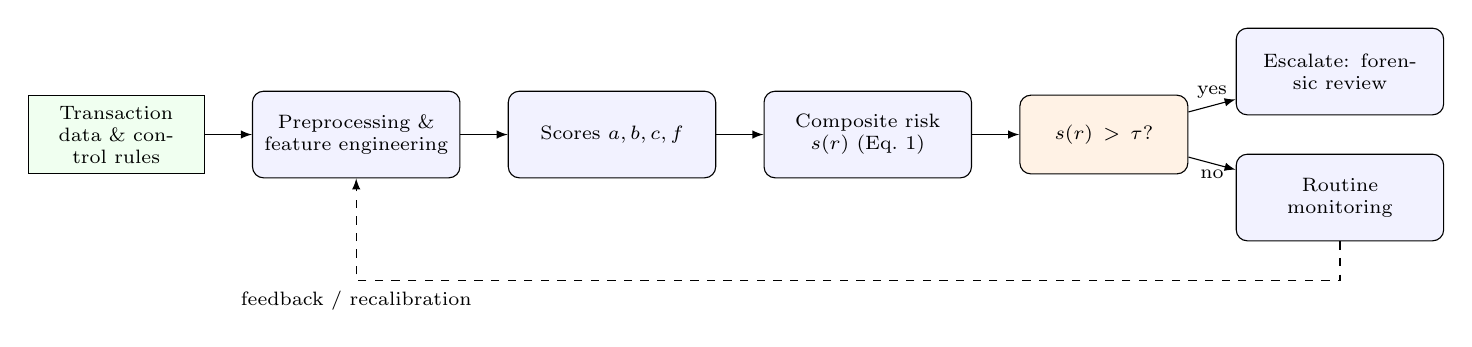
\begin{tikzpicture}[
  font=\scriptsize,
  node distance=5mm and 6mm,
  box/.style={draw, rounded corners, align=center, text width=2.4cm, minimum height=1.1cm, fill=blue!5},
  dec/.style={draw, rounded corners, align=center, text width=1.9cm, minimum height=1.0cm, fill=orange!10},
  io/.style={draw, align=center, text width=2.0cm, minimum height=1.0cm, fill=green!6},
  arr/.style={->, >=latex}]
\node[io] (data) {Transaction data \& control rules};
\node[box, right=of data] (feat) {Preprocessing \& feature engineering};
\node[box, right=of feat] (score) {Scores $a, b, c, f$};
\node[box, right=of score] (risk) {Composite risk $s(r)$ (Eq.~1)};
\node[dec, right=of risk] (thr) {$s(r)>\tau$?};
\node[box, right=of thr, yshift=8mm] (esc) {Escalate: forensic review};
\node[box, right=of thr, yshift=-8mm] (mon) {Routine monitoring};
\draw[arr] (data)--(feat);
\draw[arr] (feat)--(score);
\draw[arr] (score)--(risk);
\draw[arr] (risk)--(thr);
\draw[arr] (thr)--(esc) node[midway,above=-1pt]{yes};
\draw[arr] (thr)--(mon) node[midway,below=-1pt]{no};
\draw[arr,dashed] (mon.south) -- ++(0,-5mm) -| (feat.south) node[midway,below,font=\scriptsize]{feedback / recalibration};
\end{tikzpicture}
\caption{Conceptual AI-assisted red-flag prioritisation workflow (proposed synthesis; not empirically validated). Records above $\tau$ are escalated, others monitored, and outcomes feed back to recalibrate scores and weights.}
\label{fig:prio}
\end{figure*}

The framework is intentionally model-agnostic: each term can be instantiated with statistical, clustering, graph-based or supervised techniques reported in the literature, allowing model complexity to be matched to an organisation's data and analytical maturity. Crucially, the framework is conceptual and has not been validated in this review; no accuracy, precision or recall figures are claimed for it, and its component techniques are reported individually in the reviewed literature rather than as an integrated, evaluated system. Empirical testing is identified as a future priority in Section~\ref{sec:limitations}.

\section{Results and Discussion}
\label{sec:results}

This section synthesises the reviewed evidence around RQ1--RQ4. Throughout, we distinguish between what the reviewed sources report and our own conceptual interpretation.

\subsection{Analytical Maturity and Capability}
\label{sec:maturity}

Reported detection capability appears to be associated with analytical maturity. The reviewed literature distinguishes descriptive analytics (summarising historical patterns), diagnostic analytics (explaining the drivers of anomalies), predictive analytics (anticipating likely misconduct) and prescriptive or AI-assisted analytics (recommending actions, often using machine learning) \cite{b31,b26}. Table~\ref{tab:maturity} summarises these levels and the conditions on which they depend. Maturity is not merely a function of tooling: it is coupled with data availability and quality, workforce skills, governance and the explainability of models \cite{b32,b33}. Several sources caution that progress towards predictive and prescriptive analytics requires infrastructure investment, skilled staff and change-management effort, and that organisations in diagnostic or early predictive stages may struggle to justify prescriptive systems \cite{b34}. This suggests that maturity should be treated as a socio-technical rather than a purely technological construct---an interpretation consistent with the TOE lens adopted in Section~\ref{sec:method}.

\begin{table}[!t]
\caption{Analytics Maturity Levels and Their Reported Contribution to Audit/Fraud Workflows}
\label{tab:maturity}
\centering
\scriptsize
\begin{tabular}{p{0.18\columnwidth} p{0.36\columnwidth} p{0.30\columnwidth}}
\toprule
\textbf{Level} & \textbf{Contribution to audit/fraud workflow} & \textbf{Principal enablers / constraints} \\
\midrule
Descriptive & Retrospective reporting and population-level summarisation & Data availability; basic tooling \\
Diagnostic & Root-cause analysis of control failures and anomalies & Integrated, well-modelled data; analytical skills \\
Predictive & Risk-based prioritisation and early warning & Curated data; model validation; governance \\
Prescriptive / AI-assisted & Continuous prioritisation and response recommendation & Explainability; skills; change management \\
\bottomrule
\end{tabular}
\end{table}

\subsection{Tool-Specific Outcomes}

The synthesis of platform evidence suggests that tool effectiveness is contingent rather than absolute. Open-source analytics (Python/R) is reported to offer the greatest flexibility for complex fraud analytics and to be particularly applicable in high-risk contexts such as finance and e-commerce, where schemes may outpace rule-based detection \cite{b35,b36}. Visualisation-oriented platforms (Tableau, Power BI) are reported to support exploration and communication of financial patterns, but the reviewed sources note that they lack inherent fraud-detection capability \cite{b29}. IDEA occupies a pragmatic middle ground for file-consistency and regression-based anomaly identification, and ACL is reported as reliable for structured audit procedures because of its usability and standardised reporting, despite limited advanced detection \cite{b30}. Effectiveness is therefore conditioned by technical proficiency, data quality and the complexity of the threat \cite{b37,b12}, and combining tools may complement their individual limitations \cite{b38}. This finding supports the framework's model-agnostic design, in which no single technique is privileged.

\subsection{Red-Flag Indicators in Practice}

The five-cluster taxonomy (Table~\ref{tab:taxonomy}) is grounded in the reviewed sources. Transaction irregularities are reported as the most frequently addressed class, commonly identified through rule-based and frequency/outlier analysis \cite{b39}. Documentation discrepancies---forged, duplicated or unauthorised documents---are reported as widespread, reflecting vulnerabilities in invoice authorisation and documentary integrity \cite{b40}. Behavioural anomalies are associated with sudden changes in conduct, irregular access or resistance to oversight, and are treated as early indicators of concealed misconduct \cite{b41}. Structural anomalies arise from inconsistencies across statements, business units or reporting structures and often point to isolated controls and governance gaps \cite{b42}. Relational fraud patterns, such as bid-rigging or collusive networks, are reported as the least prevalent and most elusive, requiring graph-based analytics and cross-entity tracking \cite{b43}. Because these classes can intersect---and intersecting signals may indicate elevated risk---the synthesis supports combining multiple analytical techniques and machine-learning classifiers augmented with domain knowledge to improve sensitivity and specificity \cite{b44,b45}. We note, however, that the association between specific indicators and realised fraud is reported rather than demonstrated causally in the reviewed literature.

\subsection{Sectoral and Organisational Patterns}

Adoption and effectiveness vary across sectors, influenced by regulation, risk exposure, technological capability and organisational priorities \cite{b47}. In highly regulated sectors such as finance, healthcare and telecommunications, adoption is generally more advanced, driven by compliance mandates that favour real-time monitoring and integrated platforms \cite{b48}. In lower-resource settings---manufacturing, retail and small to medium-sized enterprises---limited budgets, weak IT infrastructure and poorly integrated data restrict adoption, leaving such organisations reliant on basic visualisation or easily implemented tools that lack the analytical depth needed for timely detection \cite{b49,b50}. Public-sector and non-profit organisations face a distinct trajectory, remaining exposed to procurement irregularities and misappropriation while implementing analytics under funding and capacity constraints \cite{b51,b52}. Across these contexts, institutional readiness, data-governance culture and alignment with objectives appear to shape assimilation more than the mere availability of technology \cite{b53}.

Comparative capability gaps between conventional and analytics-driven auditing are reported along several parameters: adaptability, staff proficiency, data infrastructure, detection speed and scalability \cite{b54,b55,b56,b57}. Whereas conventional audits rely on accounting proficiency, analytics-driven audits require combined finance and data-science expertise; organisations without targeted recruitment or training may acquire tools but struggle to extract diagnostic insight. Legacy, isolated systems compromise data integrity and limit anomaly detection, whereas integrated platforms with real-time data streams can support continuous auditing. Manual audits are bounded by human capacity, whereas analytics-driven systems offer modularity and scalability---although we interpret these advantages as reported tendencies rather than guaranteed outcomes.

\subsection{Workflow Efficacy and Governance Alignment}

Integrating analytics into audit phases is reported to accelerate procedural efficiency and responsiveness. The workflow comprises five interconnected phases---data collection, data preparation, modelling, risk assessment and red-flag generation---which function as a feedback loop rather than a linear sequence \cite{b58}. Data preparation is consistently reported as the most resource-intensive phase in terms of time and effort, and each of its steps influences model accuracy and performance \cite{b59}. Automation of routine preparation tasks, such as extract-transform-load pipelines and data-wrangling, may reduce manual effort and improve consistency \cite{b60}. Risk scoring is reported to prioritise audit activity by weightings of severity, frequency and potential financial impact, with cases above defined thresholds escalated for forensic investigation \cite{b61}. Effective governance alignment translates analytical outputs into institutional action: recurring indicators of procurement irregularities may prompt revisions to vendor-selection or approval processes \cite{b62,b63}. We interpret this as evidence that the value of analytics depends as much on governance and feedback mechanisms as on the analytical models themselves.

\subsection{Synthesis of Implementation Challenges}

The synthesis points to recurring implementation challenges that cut across sectors and tools (Table~\ref{tab:challenges}). Data quality and interoperability are repeatedly identified as the primary obstacle \cite{b15}, with data-conversion failures capable of undermining detection accuracy \cite{b25}; skill gaps affect audit teams \cite{b16}; legacy infrastructure constrains integration \cite{b49}; and algorithmic bias, fairness and transparency raise governance concerns \cite{b17,b46,b13}. Because these challenges are organisational as well as technical, mitigation is likely to require data governance, hybrid competency development and explainable-AI practices in combination, rather than tooling alone. This interpretation is consistent with the sources reviewed, although none of the reviewed studies evaluates these mitigations jointly.

\begin{table*}[!t]
\caption{Recurring Implementation Challenges and Reported Mitigations}
\label{tab:challenges}
\centering
\scriptsize
\setlength{\tabcolsep}{4pt}
\begin{tabular}{p{0.14\textwidth} p{0.35\textwidth} p{0.31\textwidth} p{0.10\textwidth}}
\toprule
\textbf{Challenge} & \textbf{Evidence reported in reviewed sources} & \textbf{Mitigation indicated in sources} & \textbf{Refs} \\
\midrule
Data quality and interoperability & Data-quality deficiencies repeatedly identified as the primary obstacle; conversion failures reduce accuracy & Standardised data governance; automated ETL/data-wrangling pipelines & \cite{b15,b25,b60} \\
Skill gaps in audit teams & Reported shortage of combined finance and data-science competencies & Hybrid competency frameworks; targeted training & \cite{b16,b55} \\
Legacy, fragmented infrastructure & Isolated, antiquated systems compromise data integrity and limit detection & Phased migration to integrated platforms; real-time data streams & \cite{b49,b53} \\
Algorithmic bias, fairness and transparency & Concerns about fairness and bias in high-stakes models; need for explainability & Bias testing; explainable AI; documented audit trails & \cite{b17,b13} \\
Tool-selection complexity & No single platform reported as universally optimal & Context-based selection aligned to objectives and competencies & \cite{b12} \\
Regulatory and standardisation uncertainty & Absence of uniform standards for algorithmic auditing & Standardised algorithmic-audit protocols & \cite{b13} \\
\bottomrule
\end{tabular}
\end{table*}

\subsection{Validation and Forward Pathways}

Triangulation across academic, professional and forensic sources supports the interpretation that analytical tools can improve audit outcomes, though it does not establish causal effects. The synthesis identifies three enduring constraints: data interoperability across platforms \cite{b64}, the need for training ecosystems covering SQL, Python and AI interpretability \cite{b65}, and regulatory clarity on algorithmic auditing and explainable AI in assurance \cite{b13}. Cross-disciplinary collaboration---between audit, IT, data science, legal and compliance functions---is indicated as important, and controlled simulation environments (``fraud sandboxes'') are proposed as a means of testing algorithmic models without legal or ethical exposure. We present these as reported proposals and our own interpretation, not as validated interventions.

\section{Conclusion and Policy Recommendations}
\label{sec:conclusion}

\subsection{Conclusion}

This review set out to synthesise fragmented evidence on business analytics for audit and fraud detection and to connect it into a coherent framework. Four things are established. First, the reviewed literature consistently associates analytics with expanded coverage (population-level testing), greater timeliness (continuous and predictive assurance) and improved traceability, relative to conventional sampling-based auditing---benefits that are reported rather than demonstrated causally in an integrative review. Second, the proposed contributions are a documented review protocol, a five-cluster red-flag taxonomy linked to analytical techniques, a comparative synthesis of five platforms with an analytics-maturity model, and a conceptual AI-assisted prioritisation framework. Third, for practitioners the synthesis offers a basis for sequencing analytics maturity, selecting tools according to objective and competency, and governing algorithmic outputs through explicit thresholds and feedback. Fourth, what remains unvalidated is the prioritisation framework itself: it is a synthesis-driven proposal whose components are reported individually in the literature but have not been evaluated as an integrated system, and no accuracy metrics are claimed for it. Accordingly, the central empirical task for future work is to test whether such a framework improves detection or triage in practice.

\subsection{Policy Recommendations}

Several implications follow for policymakers, regulators and audit leaders. First, standardising algorithmic-audit protocols would give regulators and practitioners a common basis for assurance; internationally accepted standards for AI and machine learning in auditing, with emphasis on transparent processes, are indicated \cite{b13}. Second, investment in digital audit infrastructure---upgrading legacy systems, adopting cloud-based platforms and centralised data governance---is a precondition for the integration of analytical tools. Third, competency development should be reinforced through a hybrid auditor-competency framework covering SQL, Python, inferential statistics and data visualisation, supported by professional certification and university programmes. Fourth, controlled fraud-simulation environments (``fraud sandboxes'') are proposed as regulated settings in which detection algorithms can be evaluated without legal exposure. Fifth, sector-specific implementation frameworks are needed, particularly for public-sector and non-profit organisations and SMEs, whose resource and staffing constraints differ from those of large regulated institutions. Finally, organisations should embed analytical outputs into formal governance so that identified anomalies inform upstream policy and controls.

\subsection{Limitations and Future Research}
\label{sec:limitations}

The findings are qualified by several limitations. First, this is an integrative review of secondary sources and contributes no primary empirical data; its conclusions reflect the state of the reviewed literature rather than independently measured outcomes, and no causal effects can be established. Second, the evidence base is heterogeneous, combining peer-reviewed research with industry and professional reports; although sources were tagged by type, claims resting on grey literature are weaker than those supported by peer-reviewed studies. Third, the review is subject to publication and selection bias, and coverage is weighted towards English-language sources, which may under-represent practice in other regions and languages. Fourth, the database set, while broad, is not exhaustive and excludes some specialist venues. Fifth, the proposed prioritisation framework is conceptual and unvalidated: its variables, weights and threshold are specified for clarity and testability, not as empirically fitted parameters, and the reviewed techniques are reported individually rather than as an integrated system. Sixth, the rapid pace of change in analytics and generative AI means that some tool capabilities described here will date quickly.

These limitations define a research agenda. Future work should (i) ~validate the prioritisation framework empirically using real audit datasets, reporting precision, recall and false-positive rates against a baseline; (ii) ~test its governance properties, including explainability and fairness, particularly under the bias concerns noted above; (iii) ~conduct longitudinal, multi-sector field studies to assess how analytics maturity translates into audit outcomes; and (iv) ~investigate the organisational conditions---skills, data governance and change management---that the synthesis identifies as decisive but that the reviewed literature does not evaluate jointly.

\noindent Bibliographic details were verified against public sources. Entries marked \rvr\ could not be fully confirmed and require author confirmation before submission.

\begin{thebibliography}{00}

\bibitem{b1} Ebirim, G. U., Unigwe, I. F., Oshioste, E. E., Ndubuisi, N. L., Odonkor, B., \& Asuzu, O. F. (2024). Innovations in accounting and auditing: A comprehensive review of current trends and their impact on US businesses. \emph{Int. J. Sci. Res}, 11, 965-974.

\bibitem{b2} Darwin, K. (2024). Strengthening Public and Private Accountability through Digital Forensic Accounting. \emph{Sinergi International Journal of Accounting and Taxation}, 2(4), 225-238.

\bibitem{b3} Rumasukun, M. R. (2024). Developing auditor competencies through continuous training and education. \emph{Golden Ratio of Auditing Research}, 4(1), 14-23.

\bibitem{b4} Johnson-Rokosu, S. F., \& Enobi, A. (2025). Behavioral analytics and forensic accounting: Understanding the human element in fraud. \emph{Journal of Accounting and Financial Management}, 11(5), 93-117.

\bibitem{b5} Elumilade, O. O., Ogundeji, I. A., Ozoemenam, G. O., Omokhoa, H. E., \& Omowole, B. M. (2024). Advancing audit efficiency through statistical sampling and compliance best practices in financial reporting. \emph{IRE Journals}, 7(9), 434-437.

\bibitem{b6} Nouri, Z. (2024). \emph{Financial Audit Using Data Analytics} (Master's thesis, Universidade NOVA de Lisboa (Portugal)).

\bibitem{b7} Chowdhury, R. H., \& Masum, A. A. (2025). Utilizing business analytics to combat financial fraud and enhance economic integrity. \emph{International Journal of Science and Research Archive}, 14(1), 134-145.

\bibitem{b8} Darwish, D. (Ed.). (2024). \emph{Emerging Trends in Cloud Computing Analytics, Scalability, and Service Models}. IGI Global. (ISBN 979-8-3693-0901-8)

\bibitem{b9} Ilori, O., Nwosu, N. T., \& Naiho, H. N. N. (2024). Advanced data analytics in internal audits: A conceptual framework for comprehensive risk assessment and fraud detection. \emph{Finance \& Accounting Research Journal}, 6(6), 931-952.

\bibitem{b10} Panchapakesan, A., Anandaram, H., Sridevi, L., Sathish, K. M., Dhivya, P., Parameswari, S., ... \& Kapadia, H. (2025). Enhancing Audit Effectiveness Through Strategic Data Analytics. In \emph{Machine Learning and Modeling Techniques in Financial Data Science} (pp. 231-252). IGI Global Scientific Publishing.

\bibitem{b11} Fernandes Jr, G., Rodrigues, J. J., Carvalho, L. F., Al-Muhtadi, J. F., \& Proen\c{c}a Jr, M. L. (2019). A comprehensive survey on network anomaly detection. \emph{Telecommunication Systems}, 70(3), 447-489.

\bibitem{b12} Sewpersadh, N. S. (2025). Adaptive structural audit processes as shaped by emerging technologies. \emph{International Journal of Accounting Information Systems}, 56, 100735.

\bibitem{b13} Akula, R., \& Garibay, I. (2021). Audit and assurance of AI algorithms: a framework to ensure ethical algorithmic practices in artificial intelligence. \emph{arXiv preprint arXiv:2107.14046}.

\bibitem{b14} Usul, H., \& Alpay, B. Y. (2025). Digital Transformation in Internal Audit: Paradigm Shifts, Emerging Risks, and Strategic Resilience. \emph{European Journal of Digital Economy Research}, 6(1), 23-36.

\bibitem{b15} Wolniak, R. (2024). \rvr
% [REFERENCE VERIFICATION REQUIRED: title and venue absent from the source manuscript. Candidate located: "Cybersecurity analytics: leveraging business analytics in Industry 4.0 settings", Scientific Papers of Silesian University of Technology, Organization and Management Series, No. 198, pp. 619-635; author to confirm, as its topic does not match the audit context in which the citation is used.]

\bibitem{b16} Vesty, G., Kokshagina, O., Jansson, M., Cheong, F., \& Butler-Henderson, K. (2023). Accounting, valuing and investing in health care: dealing with outdated accounting models. \emph{Meditari Accountancy Research}, 31(1), 52-77.

\bibitem{b17} Landers, R. N., \& Behrend, T. S. (2023). Auditing the AI auditors: A framework for evaluating fairness and bias in high stakes AI predictive models. \emph{American Psychologist}, 78(1), 36.

\bibitem{b18} Kothandapani, H. P. (2025). AI-Driven Regulatory Compliance: Transforming Financial Oversight through Large Language Models and Automation. \emph{Emerging Science Research}, 12-24.

\bibitem{b19} Fiolleau, K., MacTavish, C., Osecki, E., \& Thorne, L. (2024). An Exploration of Technological Innovations in the Audit Industry: Disruption Theory Applied to a Regulated Industry. \emph{Accounting Perspectives}, 23(3), 403-445.

\bibitem{b20} Hezam, Y. A., Anthonysamy, L., \& Suppiah, S. D. K. (2023). Big data analytics and auditing: A review and synthesis of literature. \emph{Emerging Science Journal}, 7(2), 629-642.

\bibitem{b21} Syam, M. A., Djaddang, S., Hasnawati, Roziq, M., \& Harnovinsah. (2025). The digital transformation of auditing: Navigating the challenges and opportunities. \emph{Economics and Business Quarterly Reviews}, 8(2), 49-66. \url{https://doi.org/10.31014/aior.1992.08.02.662}

\bibitem{b22} Faccia, A., \& Petratos, P. (2024, May). Big Data Applications in Accounting Information Systems. In \emph{Proceedings of the 2024 9th International Conference on Big Data and Computing} (pp. 1-7).

\bibitem{b23} Hassan, A., Salleh, N., Ismail, M. N., Ahmad, M. N., \& Hussin, A. R. C. (2023). Empirical evaluation of continuous auditing system use: a systematic review. \emph{International Journal of Electrical and Computer Engineering}, 13(1), 796.

\bibitem{b24} Adepoju, A. H., Austin-Gabriel, B., Hamza, O., \& Collins, A. (2022). Advancing monitoring and alert systems: A proactive approach to improving reliability in complex data ecosystems. \emph{IRE Journals}, 5(11), 281-282.

\bibitem{b25} Prosper, J. (2025). Data conversion failures and their influence on fraud detection and audit accuracy in Medicare and Medicaid. \rvr
% [REFERENCE VERIFICATION REQUIRED: no journal venue located; the work appears as a self-archived paper (ResearchGate, March 2025). Author to supply the venue or confirm it as a preprint.]

\bibitem{b26} Pamisetty, V. (2021). Integrating Predictive Analytics and IT Infrastructure for Advanced Government Financial Management and Fraud Detection. \emph{Available at SSRN 5275676}.

\bibitem{b27} Hamdam, A., Jusoh, R., Yahya, Y., Abdul Jalil, A., \& Zainal Abidin, N. H. (2022). Auditor judgment and decision-making in big data environment: a proposed research framework. \emph{Accounting Research Journal}, 35(1), 55-70.

\bibitem{b28} Abdelwahed, A. S., \& Abu-Musa, A. A. (2024). The use of big data and analytics in external auditing: Does audit firm size matter? Evidence from a developing country. \emph{South African Journal of Accounting Research}, 38(2), 113-145. \url{https://doi.org/10.1080/10291954.2023.2279751}

\bibitem{b29} Thakkar, H., Fanuel, G. C., Datta, S., Bhadra, P., \& Dabhade, S. B. (2025). Optimizing Internal Audit Practices for Combatting Occupational Fraud: A Study of Data Analytic Tool Integration in Zimbabwean Listed Companies. \emph{International Research Journal of Multidisciplinary Scope}, 6(1), 22-36.

\bibitem{b30} Pinto, A. R. O. (2024). \emph{A Framework for Leveraging it Audit Using Artificial Intelligence} (Master's thesis, Universidade NOVA de Lisboa (Portugal)).

\bibitem{b31} Lokanan, M. (2024). Harnessing exploratory data analysis for robust financial fraud detection and model enhancement. \emph{Research Square} (preprint). \url{https://doi.org/10.21203/rs.3.rs-5635767/v1}

\bibitem{b32} YV, P. K. (2021). Simple and effective descriptive analysis of missing data anomalies in smart home energy consumption readings. \emph{Journal of Energy Systems}, 5(3), 199-220.

\bibitem{b33} Machireddy, J. R. (2022). Integrating predictive modeling with policy interventions to address fraud, waste, and abuse (fwa) in us healthcare systems. \emph{Advances in Computational Systems, Algorithms, and Emerging Technologies}, 7(1), 35-65.

\bibitem{b34} Malempati, M. (2025). \emph{The Intelligent Ledger: Harnessing Artificial Intelligence, Big Data, and Cloud Power to Revolutionize Finance, Credit, and Security}. Deep Science Publishing.

\bibitem{b35} ElDahshan, K. A., Abutaleb, G. E., Elemary, B. R., Ebeid, E. A., \& AlHabshy, A. A. (2024). An optimized intelligent open-source MLaaS framework for user-friendly clustering and anomaly detection. \emph{The Journal of Supercomputing}, 80(18), 26658-26684.

\bibitem{b36} Balogun, E. D., Ogunsola, K. O., \& Samuel, A. (2021). A risk intelligence framework for detecting and preventing financial fraud in digital marketplaces. \emph{ICONIC RESEARCH AND ENGINEERING JOURNALS}, 4(08), 134-149.

\bibitem{b37} Zavarella, L. (2024). \emph{Extending Power BI with Python and R: Perform advanced analysis using the power of analytical languages}. Packt Publishing Ltd.

\bibitem{b38} Javaid, H. A. (2024). Improving fraud detection and risk assessment in financial service using predictive analytics and data mining. \emph{Integrated Journal of Science and Technology}, 1(8).

\bibitem{b39} Aivaz, K. A., Florea, I. O., \& Munteanu, I. (2024). Economic Fraud and Associated Risks: An Integrated Bibliometric Analysis Approach. \emph{Risks}, 12(5), 74.

\bibitem{b40} Nogueira, D. M., Sim\~oes, M., Ferreira, C., Ribeiro, R. P., Mart\'inez-Rego, D., Cai, A., \& Gama, J. (2025). Survey on Detection of Fraudulent Documents. \emph{Authorea Preprints}.

\bibitem{b41} Douglas, F. (2024). \emph{Can Small Businesses Deter Fraud? A Qualitative Examination of Preventive and Detective Internal Control Strategies} (Doctoral dissertation, National University).

\bibitem{b42} Qatawneh, A. M. (2024). The role of artificial intelligence in auditing and fraud detection in accounting information systems: moderating role of natural language processing. \emph{International Journal of Organizational Analysis}.

\bibitem{b43} Hilal, W., Gadsden, S. A., \& Yawney, J. (2022). Financial fraud: a review of anomaly detection techniques and recent advances. \emph{Expert systems With applications}, 193, 116429.

\bibitem{b44} Popoola, N. T. (2023). Big data-driven financial fraud detection and anomaly detection systems for regulatory compliance and market stability. \emph{Int. J. Comput. Appl. Technol. Res}, 12(09), 32-46.

\bibitem{b45} Adejumo, A., \& Ogburie, C. (2025). Financial statement manipulation: Ethical and regulatory perspectives. \emph{GSC Advanced Research and Reviews}, 22(03), 252-264.

\bibitem{b46} Baeyaert, J. (2025). Harmonizing creativity and ethics in AI systems. \emph{AI and Ethics}, 1-21.

\bibitem{b47} Bello, H. O., Ige, A. B., \& Ameyaw, M. N. (2024). Adaptive machine learning models: concepts for real-time financial fraud prevention in dynamic environments. \emph{World Journal of Advanced Engineering Technology and Sciences}, 12(02), 021-034.

\bibitem{b48} Sutisna, E. (2025). Evaluating Security Risks and the Impact of Analytic Technology on the Audit Process. \emph{Advances in Managerial Auditing Research}, 3(1), 30-43.

\bibitem{b49} Akter, M. (2025). \emph{Enhancing SME Competitiveness: The Role of Business Intelligence in Data-Driven Decision-Making} (Bachelor's thesis). Theseus repository (URN:NBN:fi:amk-202504227203).

\bibitem{b50} Ayodeji, I. A. (2024). \emph{Fraud Detection and Prevention in the Nigerian Financial Industry} (Doctoral dissertation, Walden University).

\bibitem{b51} Pizzini, M., \& Sterin, M. (2025). The relation between cash reserves, governance, and donations in nonprofit organizations. \emph{Journal of Accounting, Auditing \& Finance}, 40(1), 139-164.

\bibitem{b52} Alex-Omiogbemi, A. A., Sule, A. K., Omowole, B. M., \& Owoade, S. J. (2024). Conceptual framework for advancing regulatory compliance and risk management in emerging markets through digital innovation. \emph{World Journal of Advanced Research and Reviews}, 24(3), 1155-1162. \url{https://doi.org/10.30574/wjarr.2024.24.3.3752}

\bibitem{b53} Solano, M. C., \& Cruz, J. C. (2024). Integrating analytics in enterprise systems: A systematic literature review of impacts and innovations. \emph{Administrative sciences}, 14(7), 138.

\bibitem{b54} Wagener, M., Eulerich, M., \& Bonrath, A. (2025). From Pen-and-Paper to Technology-Driven Analytics: Technology Usage in Internal Auditing. \emph{Journal of Information Systems}, 1-28.

\bibitem{b55} Oliveira, J., \& Ribeiro, P. J. (2022). Technological developments and new hybrid roles in accounting and finance. In \emph{The Routledge Handbook of Accounting Information Systems} (pp. 156-170). Routledge.

\bibitem{b56} Naoufal, G. (2024). Continuous auditing/continuous monitoring. In \emph{Continuous Auditing with AI in the Public Sector} (pp. 143-162). CRC Press.

\bibitem{b57} Oko-Odion, C., \& Udoh, O. R. (2024). Leveraging technology in internal audit processes for streamlined management and risk oversight. \emph{International Journal of Science and Research Archive}, 13(2), 3077-3100. \url{https://doi.org/10.30574/ijsra.2024.13.2.2549}

\bibitem{b58} Ruhnke, K. (2023). Empirical research frameworks in a changing world: The case of audit data analytics. \emph{Journal of International Accounting, Auditing and Taxation}, 51, 100545.

\bibitem{b59} Joshi, A. P., \& Patel, B. V. (2021). Data preprocessing: the techniques for preparing clean and quality data for data analytics process. \emph{Orient. J. Comput. Sci. Technol}, 13(0203), 78-81.

\bibitem{b60} Vajpayee, A. (2023). The Role of Machine Learning in Automated Data Pipelines and Warehousing: Enhancing Data Integration, Transformation, and Analytics. \emph{ESP Journal of Engineering \& Technology Advancements}, 3(3), 84-96.

\bibitem{b61} Henriques, J. P. M. (2024). \emph{Audit Compliance and Forensics Frameworks for Improved Critical Infrastructure Protection} (Doctoral dissertation, Universidade de Coimbra).

\bibitem{b62} Carre\~no, A. M. (2024). Strategic alignment in program management: A framework for sustainable business transformation. Institute for Change Leadership and Business Transformation. \rvr
% [REFERENCE VERIFICATION REQUIRED: only an institute/professional source (ICLBT) and a ResearchGate record were located; peer-review status unclear. Author to confirm.]

\bibitem{b63} Sarkola, M. (2023). \emph{Developing global system-based indirect purchasing in the case company} (Master's thesis, LUT University).

\bibitem{b64} Mai, L. P. (2022). \emph{Changes in competencies, capabilities, and decision-making in the accounting profession as a result of information digitalization and big data analytics/artificial intelligence} (Master's thesis, Ca' Foscari University of Venice).

\bibitem{b65} George, J. (2022). Optimizing hybrid and multi-cloud architectures for real-time data streaming and analytics: Strategies for scalability and integration. \emph{World Journal of Advanced Engineering Technology and Sciences}, 7(1), 174-185.

\bibitem{b66} Cressey, D. R. (1953). \emph{Other People's Money: A Study in the Social Psychology of Embezzlement}. Glencoe, IL: Free Press.

\bibitem{b67} Tornatzky, L. G., \& Fleischer, M. (1990). \emph{The Processes of Technological Innovation}. Lexington, MA: Lexington Books.

\end{thebibliography}

\end{document}
